\section{Introduction}
\label{sec:introduction}

Under the critical fugacity law, the length is not prescribed: each extra step is penalized by its critical fugacity, while the number of possible paths grows. In a bounded domain these effects balance to produce a nontrivial mean length. We study that mean for paths joining the boundary of an equilateral triangle. The two endpoints are summed over, and a diameter restriction selects paths that explore a fixed fraction of the domain.

Let $\mathbb H$ be the honeycomb lattice dual to the tiling by unit equilateral triangles. A \emph{port} is the midpoint of a side of a tiling triangle. A port-to-port path joins successive ports through triangle centres, visits each centre at most once, and has distinct initial and final ports. Its length $m(\gamma)$ is its number of visited centres. We use
\[
 x=(2\cos(\pi/8))^{-1}=(2+\sqrt2)^{-1/2},
 \qquad w(\gamma)=x^{m(\gamma)}.
\]
An ordinary centre-to-centre walk visiting $m$ centres has $m-1$ edges, so changing between these two length conventions changes every path weight by the same factor $x$.

For an integer $R\ge1$, let $\Delta_R$ be the closed equilateral triangle of side length $R$ made of tiling triangles. Write $\mathcal C_R$ for the port-to-port paths inside $\Delta_R$ whose initial and final ports belong to its boundary and whose Euclidean diameter is at least $R/100$. We count both endpoint orders; using unoriented paths gives the same probability measure after the factor two cancels. Define
\[
 Z_R^{\rm chord}=\sum_{\gamma\in\mathcal C_R}w(\gamma),
 \qquad
 \mathbb P_R(\gamma)=\frac{w(\gamma)}{Z_R^{\rm chord}}.
\]
Here and below $f(R)\asymp g(R)$ means that their ratio lies between two positive constants for all sufficiently large $R$. The notation $f(R)=R^{a+o(1)}$ means $\log f(R)/\log R\to a$.

\begin{theorem}[Macroscopic triangle chords]\label{thm:triangle}
For the critical chord law $\mathbb P_R$,
\[
 Z_R^{\rm chord}\asymp R^{3/4},
 \qquad
 \mathbb E_R m=R^{4/3+o(1)}.
\]
The same mean exponent holds for ordinary centre-to-centre self-avoiding walks contained in $\Delta_R$, with both endpoints on its inner boundary layer (the centres adjacent to a boundary port), weighted by $x$ per edge and restricted to have diameter at least $R/100$.
\end{theorem}

This is a statement about the mean under a law that sums both endpoints and every admissible length. Prescribing two ports changes the normalization and requires additional estimates. Likewise, a mean alone does not give a matching lower bound on the typical length. Those distinctions matter because the present proof extracts an integrated contact mass rather than a concentration estimate.

The exponent $4/3$ is the reciprocal of the predicted size exponent $\nu=3/4$ for a uniformly chosen $n$-step honeycomb walk, whose mean-square endpoint displacement is predicted to be $n^{2\nu+o(1)}$~\cite{DuminilCopinSmirnov2012}. This is a heuristic comparison of scales: the fixed-length displacement law differs from the finite-triangle critical law considered here. A related rigorous estimate of Krachun and Panagiotis bounds the maximal distance from the starting point of a uniform $n$-step honeycomb walk by $O(n/\log n)$ with probability tending to one~\cite{KrachunPanagiotis2026}; it does not determine the finite-triangle mean.

\subsection{Critical weights and the amplitude problem}

Nienhuis's dilute $O(n)$ calculation identified the critical point and the associated critical-exponent predictions for planar loop models~\cite{Nienhuis1982}. Duminil-Copin and Smirnov proved that the honeycomb connective constant is $\sqrt{2+\sqrt2}$, using a parafermionic observable whose local cancellation controls boundary path sums~\cite{DuminilCopinSmirnov2012}. We use that local cancellation in a finite exploration form. Including the tangent factor in their observable of spin $5/8$ gives the flux exponent $1-5/8=3/8$ used here. Its phases will be kept explicit, because changing from an exterior source to an interior slit changes the surviving loop weight.

The local transfer matrices belong to the dilute integrable-model setting. Their exchange and fusion identities permit changes of row arguments and of circumference. Grimm and Pearce~\cite{GrimmPearce1993} give the dilute braid--monoid construction; Zhou and Batchelor~\cite{ZhouBatchelor1997} analyze periodic spectra and the seam weight in the dilute $O(n)$ and Izergin--Korepin setting. Glazman and Manolescu prove boundary two-point invariance for columnwise rhombic half-plane tilings with angles in $[\pi/3,2\pi/3]$ and Yang--Baxter walk weights~\cite{GlazmanManolescu2017}. These results explain the usefulness of deforming local weights while preserving finite identities. In this paper the local matrix identities are proved in the precise gauge used by the boundary states.

The main analytic obstacle is a boundary coefficient. If a finite transfer matrix $T$ has a simple dominant eigenvalue $\lambda$, then a matrix element between two fixed boundary states has leading form
\[
 \Lambda T^H\Psi=c\lambda^H+\text{smaller terms}.
\]
Knowing $\lambda$ does not determine $c$: the coefficient depends on both boundary states. Earlier integrable honeycomb adsorption boundaries were studied by Batchelor and Yung~\cite{BatchelorYung1995}; the caps considered here have their own contraction and normalization. Here $\Psi$ and $\Lambda$ are vacuum states that suppress closed loops outside the marked region. Their twists differ from the twist of the rows between them. The residue formula and the physical selection argument determine this coefficient in the required normalization.

\subsection{The positive observables behind the proof}

Two polygon sums connect this coefficient to Theorem~\ref{thm:triangle}. The first is planar. Fix a vertex $v$ of the triangular tiling, equivalently a face centre of $\mathbb H$. Let $\mathcal Z_v(r)$ be the sum over finite collections of pairwise vertex-disjoint simple honeycomb polygons, each enclosing $v$ and lying within Euclidean distance $r$ of $v$. A polygon $P$ has weight $2x^{|P|}$, where $|P|$ is its number of edges, and the empty collection has weight one. Such collections are necessarily nested.

For the cylinder, orient the tiling with horizontal sides and group its
triangles into rows of $\pi/3$-rhombi, whose sides are parallel to $0$
and $\pi/3$. The row index increases by one under translation by
$e^{i\pi/3}$. For an integer $N\ge1$, identify horizontal translates
by $N$. Choose a seam along the row direction between neighboring
columns, with tips at the cuts of integer heights $0$ and $H\ge0$.

Let $\mathcal G_N(H)$ be the sum over finite collections of pairwise
vertex-disjoint simple honeycomb polygons on this cylinder of two kinds:
winding polygons separating the tips, and contractible polygons
enclosing exactly one tip. Each polygon $P$ has weight $2x^{|P|}$,
and the empty collection has weight one. Define the sum by exhaustion
in both row directions.

For comparison, let $L_N(H)$ be the winding-only partition function
between the height cuts $0$ and $H$, with no polygon crossing either
cut. Its polygons are contained in the slab, have the same weights,
and the empty collection is included. Write
\[
 \lambda_N:=\lim_{H\to\infty}L_N(H)^{1/H}.
\]
Section~\ref{sec:projection} proves that this limit exists and identifies
it with the positive row growth factor. The following result states the
cap amplitude and planar nesting estimates in these conventions.

\begin{theorem}[Cylinder amplitude and planar nesting]\label{thm:amplitude}
For each sufficiently large $N$, the preceding cylinder sums are finite and
\[
 \mathcal A_N:=\lim_{H\to\infty}\lambda_N^{-H}\mathcal G_N(H)
 \quad\text{exists in }(0,\infty).
\]
Their asymptotics and the planar nesting asymptotic are
\[
 \mathcal A_N=N^{1/6+o(1)},
 \qquad \mathcal Z_v(r)=r^{1/12+o(1)}.
\]
The bounds are unchanged by a lattice translation of $v$.
\end{theorem}

\begin{figure}[t]
\centering
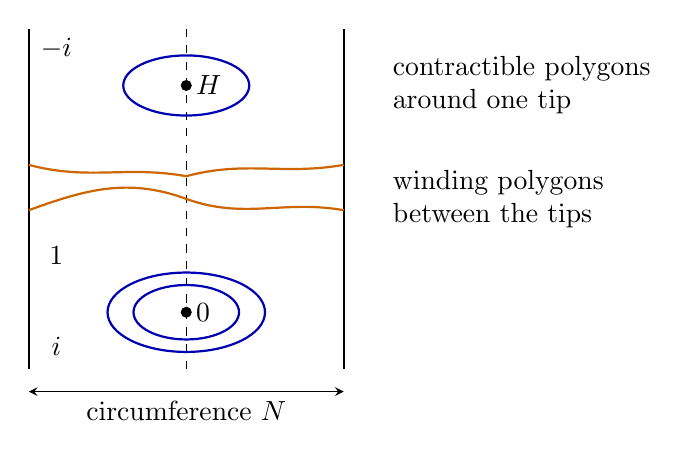
\begin{tikzpicture}[x=1cm,y=.72cm,>=stealth]
\draw[thick] (0,0)--(0,6) (4,0)--(4,6);
\draw[dashed] (2,0)--(2,6);
\fill (2,1) circle(2pt) node[right] {$0$};
\fill (2,5) circle(2pt) node[right] {$H$};
\node at (.35,.4) {$i$};
\node at (.35,2) {$1$};
\node at (.35,5.65) {$-i$};
\draw[blue!70!black,thick] (2,1) ellipse(.67 and .48);
\draw[blue!70!black,thick] (2,1) ellipse(1 and .7);
\draw[blue!70!black,thick] (2,5) ellipse(.8 and .53);
\draw[orange!80!black,thick] (0,2.8) to[out=20,in=160] (2,3) to[out=-20,in=170] (4,2.8);
\draw[orange!80!black,thick] (0,3.6) to[out=-15,in=170] (2,3.4) to[out=15,in=190] (4,3.6);
\draw[<->] (0,-.4)--(4,-.4) node[midway,below] {circumference $N$};
\node[align=left,anchor=west] at (4.5,5) {contractible polygons\\around one tip};
\node[align=left,anchor=west] at (4.5,3) {winding polygons\\between the tips};
\end{tikzpicture}
\caption{A schematic fundamental rectangle for the cylinder: its vertical sides are identified. The dashed seam has tips at cuts $0$ and $H$; the labels $i$, $1$, and $-i$ give its twist in the three row regions. The surviving contractible polygons enclose one tip, and the surviving winding polygons separate the tips. Dividing by the winding growth retains the two tip contributions. Curves are schematic and do not represent individual lattice edges.}
\label{fig:seam}
\end{figure}


The factor two between these exponents has a geometric meaning. When the seam tips are far apart, each tip supports a planar nest, while the winding polygons lie between them. The transfer coefficient records the two tip contributions after the extensive winding growth $\lambda_N^H$ has been removed. Proving this comparison requires height bounds: a cylinder polygon can be too tall, or its planar lift too wide, to belong to a small neighbourhood of one tip. We establish moments of every fixed order before making the projection.

\subsection{A complete route through the argument}

The proof begins with positive path sums. Section~\ref{sec:local} proves the local matrix identities, and Section~\ref{sec:cylinder} converts them into two estimates: a cylinder boundary deficit of order $N^{-1/4}$ and winding-polygon mass of order $N^{-1}$ per highest row. The deficit is the eventual source of the chord normalization $R^{3/4}$.

Sections~\ref{sec:vacuum}--\ref{sec:repeated-moments} determine the coefficient selected by the two caps. We first construct their normalized vectors and their polynomial denominator. A scalar residue formula then expresses products of row transfers between the caps, with an explicit normalization for the empty product. The root twists are initially independent. Resolving collisions proves that the scalar trace is holomorphic near a generic common twist, where colliding roots may contribute derivatives as well as ordinary evaluations. Adding and removing fused pairs of sites then extends the identity from distinct site arguments to arbitrary repeated row arguments by meromorphic continuation. This step is needed to compute powers $T^H$, not just a finite collection of special matrix elements.

Sections~\ref{sec:counting}--\ref{sec:asymptotics} identify the physical term in that formula. A real counting system has a unique branch in explicit quantile boxes, including the two extreme roots. Polynomial orthogonality identifies the vacuum end of the branch. Positivity of the finite annular transfer and a separate estimate on the two boundary caps select its ordinary residue coefficient at generic parameters. The finite annular gap and cap estimate make the selected coefficient analytic near each point of this real branch, so the identity continues to the homogeneous physical endpoints. The coefficient is a ratio $W/J$ of a root product and a Jacobian determinant, normalized at zero winding fugacity. Its logarithmic asymptotics give the exponent $1/6$.

Section~\ref{sec:projection} obtains arbitrary fixed height moments from higher twist derivatives, projects the cylinder polygons to the plane, and proves Theorem~\ref{thm:amplitude}. Section~\ref{sec:chords} completes the positive walk argument. An edge-slit exploration compares the weight of chords visiting an interior contact with the surrounding polygon partition. That contact weight is at most $R^{1/12+o(1)}$ everywhere and has this order throughout a central region. Summing order $R^2$ contacts gives the unnormalized length mass $R^{25/12+o(1)}$. The boundary deficit gives $Z_R^{\rm chord}\asymp R^{3/4}$, and their ratio is the exponent in Theorem~\ref{thm:triangle}.

The angle $l=\pi/8$ is fixed throughout; integer shifts inside bracketed trigonometric formulas denote multiples of $l$, whereas geometric row heights are integers in the physical lattice.
